\documentclass{stylesheet}

\usepackage{color}
\usepackage{url}
\usepackage{enumerate}
\usepackage{verbatim}
\usepackage[english]{babel}%spell check
\usepackage[colorinlistoftodos]{todonotes}%todo
\usepackage{etoolbox}%Remove the ugly copyright from the template :-)
\makeatletter%Remove the ugly copyright from the template :-)
\patchcmd{\maketitle}{\@copyrightspace}{}{}{}%Remove the ugly copyright from the template :-)
\makeatother%Remove the ugly copyright from the template :-)

\usepackage[nameinlink,capitalise]{cleveref}

\begin{document}
\title{Cloud Computing}

\numberofauthors{5} 
\author{
% 1st. author
\alignauthor
Christos Froussios\\
	\affaddr{4322754}\\
	\email{C.Froussios @student.tudelft.nl}
% 2nd. author
\alignauthor
Richard van Heest\\
	\affaddr{4086570}\\
	\email{A.W.M.vanHeest @student.tudelft.nl}
\and
% Alex
\alignauthor
Alexandru Iosup\\
	\affaddr{Course instructor}
	\email{A.Iosup@tudelft.nl}
% Dick
\alignauthor
Dick Epema\\
	\affaddr{Course instructor}
	\email{D.H.J.Epema@tudelft.nl}
% Alexey
\alignauthor
Alexey Ilyushkin\\
	\affaddr{Teaching Assistant}
	\email{A.S.Ilyushkin@tudelft.nl}
}

\maketitle

\begin{abstract}
Cloud computing has been increasingly popular over the last decade. It seems promising in some ways, given the successes with cloud based systems of some large companies. However, there are drawbacks on this kind of systems as well. In this report we describe our findings of one month of research in the area of cloud computing. We build a small prototype of a IaaS-based application that does image processing and runs on the Amazon Web Services (AWS) EC2 cloud platform. The main focus points in the design and research of this prototype are automation, scalability, load balancing, reliability and monitoring. To solve issues like scalability and load balancing, we develop several policies to be tested and compared against each other. Furthermore we measured the performance of the system by applying several metrics. Finally we come up with an analysis of the pro's and con's of switching to cloud computing.
\end{abstract}

\section{Introduction}
Cloud computing has gained an increasing interest in the last couple of years. In contrast to the era of grid computing, not only the academic world is interested in this new way of performing large scale computations, but also companies do so. The most logic explanation for this shift of interest is that computer grids are expensive to invest in for a company which may not use the required hardware constantly, whereas in cloud computing that company would lease the required machines, scale up or down if appropriate and only get charged for the hours between leasing and releasing.

We distinguish three types of cloud computing:
\begin{description}
	\item[Software as a Service (SaaS)] applications such as Google Drive, Dropbox, Gmail, Yahoo mail and Facebook.
	\item[Platform as a Service (PaaS)] the computing platforms which typically include operating systems, programming language execution environments, databases and web servers. Examples of this are Apache Hadoop, Google App Engine, Windows Azure and Amazon Web Services Elastic Beanstalk.
	\item[Infrastructure as a Service (IaaS)] the computing infrastructure, physical or (more often) virtual machines and other resources like virtual-machine disk image libraries, block and file-based storage, firewalls, load balancers, IP addresses and virtual local area networks. The most prominent products in this category are Windows Azure, Google Compute Engine and Amazon EC2.
\end{description}

In this report we will focus on IaaS cloud computing especially, as requested to investigate by WantCloud BV. We will look into the advantages and disadvantages of IaaS by implementing a small prototype for a potential future system. The main features of this prototype can be summarized as:
\begin{description}
	\item[Automation] working as much as possible independently from any human interaction
	\item[Elasticity (auto-scaling)] leasing and releasing machines from a resource pool as workloads change over time
	\item[Performance (load balancing)] allocating workloads to machines from the resource pool in such a way that the machines are used as effective as possible.
	\item[Reliability] building in a fair amount of fault tolerance
	\item[Monitoring] observing and recording the current status of the system as well as measuring its components' performance by applying various metrics.
	\item[Multi-tenancy] having multiple concurrent users in the system while discriminating between their importance.
\end{description}

The prototype to be implemented will be an application that receives pictures from an external source (for example a web form where users can submit their pictures), performs some operations on them and returns the processed pictures. These operations may vary from lightweight operations such as a flip of the picture to heavier operations like Fourier transform.

The application is set up in such a way that all pictures are received at a head node, which allocates them to one of the worker node in its resource pool and leases new machines or releases idle machines when appropriate. We present and compare multiple policies for these problems.

This report is structured as follows: first we will discuss the background of the application in \cref{sec:background}. What does it do in detail? What are its requirements and features? This is followed by the system design in \cref{sec:design}, where we focus on the internal workings of the application as well as several policies for both the processes of allocation and leasing/releasing nodes. We evaluate the application in \cref{sec:experiments} by applying several metrics. Finally we close the report with a discussion in \cref{sec:discussion} and the conclusion in \cref{sec:conclusion}. In \cref{app:time} an overview of spent time is provided.

\section{Background of the application}
\label{sec:background}
The application we build over the course of several weeks is a prototype of a more generic cloud centered solution where tasks come in at the head node and are distributed over a number of worker nodes. In this particular application we choose to take image processing as the workload. Pictures that are received by an arbitrary worker are modified by applying a number of operations, combining them afterwards. Notice that this approach has a high potential for the task being split into subtasks and make it into a MapReduce process. However, to make things not overly complicated in this prototype, we consider one picture as one \textit{undividable} task, which is executed on a single node.

The basic requirements of our application can be split up into 5 tiers. First of all, the application needs to run without human intervention as much as possible. We fulfilled this requirement by only having to start the head node application and providing pictures over the course of the runtime. Besides these 2 acts, the head node automatically decides when to lease and release worker nodes, to which worker an incoming task is sent and to where a completed task needs to be returned. On the other hand, the worker nodes automatically receive tasks, process them as soon as they possible can and make sure they send back the result to the head node.

A second tier holds the elasticity (or scalability) of the system, which is determined by the head node. Elasticity in the context of cloud computing describes to which degree the system is able to grow and shrink its number of resources. In this case, these resources are the worker nodes, which can be leased or released. When the system gets overloaded with tasks, it might be a good idea to lease more workers. On the other hand, when there are hardly any tasks in the system, it is useless to have a large number of idle workers, since they are being payed for all that time. Ideally you want to predict when the system will have a peak moment in the number of tasks and when it will get more quiet. For this, machine learning is a nice path to follow. This however is not part of this project.

Besides elasticity, load balancing is another topic of interest in cloud computing. When the head node receives a task, it needs to decide where it should be executed. Does it prefer certain workers, will it be assigned randomly or is there a better way to schedule a task. In this the head node might look at the size of the task, the length of the queue of each available worker or any other measurable property of the task and the workers.

The fourth tier is the reliability of the system. As the application is mostly autonomous, it also needs to be able to recover itself from failure. A failure might be losing connection between the head node and one or more workers, crashing the head or a worker, IO failure, etc. For this project we make the assumption that the head node never crashes and that it never completely loses access to the network.

Finally, a system isn't a good system without a monitoring module. To make decisions in the other tiers (especially elasticity and load balancing), we need to supply it with proper data, for example the length of each worker's queue, the number of incoming tasks in the system, etc. Also for the research part of this project the monitoring module is used. This is used to gain the results in \cref{sec:experiments}.

Besides these 5 tiers, we added support for multi-tenancy. It is possible for multiple users to connect to the head node and send in their images. At this point, the system does not discriminate between the importance of users and uses the policy of ``First-come, first-served''.

\section{System Design}
\label{sec:design}
The application we present here can be seen as a prototype for a typical cloud centric work flow, where a user sends workloads to a head node, which distributes it over one or more workers (depending on whether the workloads are splittable into subtasks). Once the workload is processed, a result is send back to the head node, which forwards this result to the appropriate user. Based on the workloads, the head node needs to decide to which worker a workload is allocated and whether or not to lease or release workers, for which it uses certain policies.

In this section we will discuss the system's architecture, work flow, communication between user, head node and workers, followed by the policies that are used in scaling and load balancing. Finally we will describe the additional features that is in the system: multi-tenancy. Where possible we will give a more general description of the design, rather than describing the system for the current image processing application. This might help in developing future projects based on the same principle.

\subsection{Architectural overview}
\label{subsec:resourceManagement}
In order to understand the system's architecture and work flow, let's follow a workload as it works its way through the system. We refer to \cref{fig:headnode} and \cref{fig:worker} for an overview of the architecture.

The user who sends this workload will sign in to the head node via a socket connection. This connection request comes in at the \texttt{ClientReception}, which creates a \texttt{ClientHandle} for workloads to be received. From this point on, the user interacts directly with its own \texttt{ClientHandle} in the head node. When this receives a workload, it makes a local copy of the workload and adds it to the \texttt{TaskQueue}. This is where all workloads come together while waiting to be processed. It should be noted that (for reasons explained later) the \texttt{TaskQueue} is a double-ended queue, meaning that tasks not only can be pushed at the end of the queue but also at the beginning.

\begin{figure*}
	\centering
	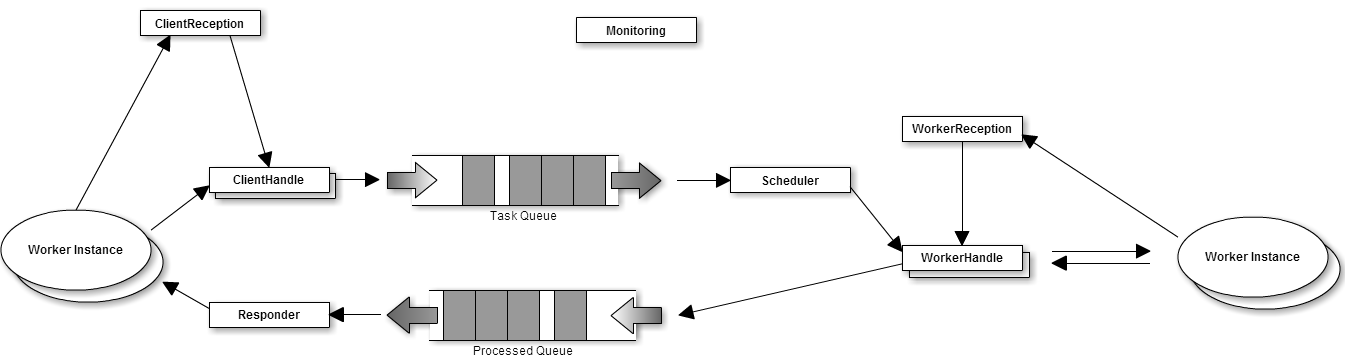
\includegraphics[width=\textwidth]{Architecture_head.png}
	\caption{Architecture in the head node}
	\label{fig:headnode}
\end{figure*}

\begin{figure*}
	\centering
	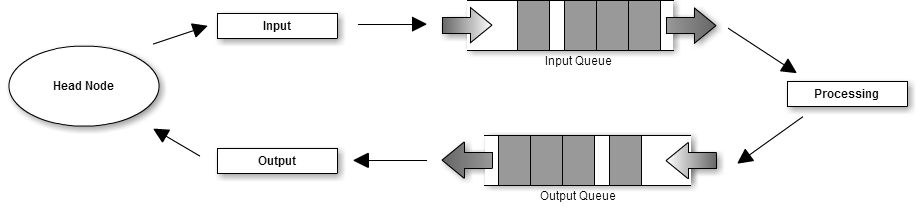
\includegraphics[width=0.8 \linewidth]{Architecture_worker.png}
	\caption{Architecture in a worker}
	\label{fig:worker}
\end{figure*}

The \texttt{Monitor} continuously samples the current state of the head node. For this reason, it also knows that the workload is queued. Based on the total workload in the queue (and other metrics and policies that are explained later), it decides whether or not to lease extra workers. When extra workers are needed, the \texttt{Monitor} makes a call to the Cloud Service to request a new machine.

The \texttt{WorkerReception} waits for this machine to contact the head node. Once the socket connection is established, a \texttt{WorkerHandle} is created and stored in the head node, via which all future communication with the newly leased machine will take place. The first communication is the worker who introduces itself and tell how many cores it has. This information is stored in the \texttt{WorkerHandle} for later use. Once this formal procedure is over, the new worker will wait for the first workloads to come in.

Besides coordinating the leasing of workers, the \texttt{Monitor} is also responsible for cleaning up workers that are not needed anymore. This is done based on metrics and policies that will be discussed later. When it decides to release a worker, the corresponding {\verb WorkerHandle } will be flagged as being set for decommission. After that, no more tasks can be scheduled on that worker; it will only finish its currently scheduled tasks, after which is is released.

The \texttt{Scheduler} takes workloads out of the \texttt{TaskQueue} and decides on which workers they will be processed. This subsystem takes all tasks out of the queue and collects all eligible workers (the ones that are not flagged for decommission). Based on a predefined policy, an allocation plan is made where tasks are assigned to certain workers. It is possible in some policies that not all tasks can be scheduled at once. For that reason, not only the allocation plan is returned by the policies, but also a list of not yet scheduled tasks. The latter will be put back on top of the queue, so that they are the first to be scheduled again next time. The tasks that were in the allocation plan will get assigned to the appropriate workers by sending their workloads over the previously established socket connection. In the case the connection failed in the meantime, the task is put back in the queue as well to be rescheduled.

When a task is allocated to a certain worker, its workload will be send over there via the socket connection. At the worker side, it is received by the \texttt{Input} subsystem, which puts it in the \texttt{InputQueue} for it to be processed. When the \texttt{Processing} subsystem is finished with the previous task, it will take the workload out of the queue and performs the actual processing. After that is finished, the result is put into the \texttt{OutputQueue}, from where it is send back to the head node by the \texttt{Output} subsystem.

At the head node, the result is received over the socket  by the \texttt{WorkerHandle} which removes the corresponding task from the list of currently processed jobs and adds the result to the \texttt{ProcessedQueue}. There it waits until the \texttt{Responder} takes it out and sends it back to the user.

\subsection{Architectural future improvements}
The architecture described above is what the application currently looks like. However, this does not fully satisfy the redundancy requirement. This is due to this project's deadline. In the following we describe what to change in and add to the architecture to fully support this requirement.

The head node is the system's single point of failure. To defend against failures in the head node, the node can be mirrored. Despite being significantly lighter than worker nodes, the head node can also be overwhelmed in a busy real environment. To improve scalability, it is possible to split the head's components into a set of closely collaborating nodes. In that case, only the scheduler and monitor need to be mirrored. Other components can naturally collaborate with duplicates of themselves.

When the connection to a worker fails, the head node removes that worker from the worker pool and continues serving requests using the rest of the workers. All the tasks assigned to that worker are presumed lost. If the failure was temporary, the worker is responsible for re-initiating connection to the head node and re-entering the worker pool as a new worker. In the current state of our implementation, workers do not attempt to recover. This was not deemed necessary, as such failures are so rare (we did not encounter any) that we did not consider them a significant resource leak. In a more robust implementation, a worker should attempt to publish its log files and stop, so as not to sit idle.

As we already said, tasks assigned to a failed worker are presumed lost, since one cannot reliably expect the worker to recover on time. That leaves us with the problem of resuming work on a different worker, in the case that the head node does not have enough RAM memory to backup every request, or enough storage IO bandwidth to store them on a local drive. For that, we would propose a third node role: the file node. That node serves as a remote hash map, that stores tasks given to it and serves them when requested with their unique id. The head node, upon receiving a request, passes it on to one or more file nodes to be stored. When scheduling the task, rather than transmitting the workload, only the identifier and a list of file nodes is sent. The worker then retrieves the workload from the closest available worker. The result of the task is then returned to the file nodes and the head is signaled to retrieve it and send the response.

Since the file node is an IO-heavy process, while the worker node is CPU-heavy, it is recommended that both are deployed on each machine to maximize the use of the machine's resources. That has the additional advantage that if the file node that holds a task and the worker that has to process it are on the same machine, loading the image is done locally and network resources are preserved. A special task scheduler can be designed so that it shows preference to the worker that resides next to a file node that holds the task.

\subsection{System policies}
\label{subsec:policies}
When it comes to scheduling tasks or leasing and releasing workers, the approach can influence the performance of the whole system. In this section we discuss the different policies we created for both scheduling, leasing and releasing.

\subsubsection*{Scheduling policies}
Every scheduling policy implementation receives a list of tasks to be scheduled as well as a collection of eligible workers and has to return both an allocation plan and a list of unscheduled tasks. We first present some simple policies, followed by some more sophisticated policies that are all scheduling all provided tasks. After that, we modify the latter policies to only schedule some of the tasks while rejecting others.

A very basic scheduling policy, the \texttt{RoundRobinScheduler}, does not need any knowledge about the workers or the tasks. It allocates the tasks by iterating over the collection of workers. It treads every worker and every task in an equal way, giving no priority to any of the tasks and not regarding the length of the queue of a certain worker.

A modification of this policy would be to not iterate over the collection of workers but instead allocate the tasks randomly to certain workers, hence the name \texttt{RandomScheduler}. This might cause an unbalance in the distribution of tasks on a single scheduler run, but given simple statistical methods and theorems it will ultimately give a more balanced solution in the long run.

The previous policies might be used when the scheduler for particular reasons is not allowed or able to know the current state of the workers or the contents of the tasks. However, when this restriction is not there, an obvious more sophisticated policy is the \texttt{QueueLengthScheduler}, which makes the allocation decision based on the number of tasks that are already present in that worker. The worker with the least amount of tasks will be the one to execute the task at hand. This however asks either for a lot of communication with each of the workers to check their status or a good bookkeeping solution in the head node. The decision for this trade-off can be based on the amount of computer memory versus the speed of the communication. Also this policy assumes that all tasks are of equal processing length, which is more than often not the case.

A `\textit{future work}' policy that takes this processing length into account is the \texttt{QueuePixelScheduler}. This is a somewhat special policy for our case of image processing that follows from the way our image processing is implemented and can be summarized by the conclusion that the number of pixels in a picture is proportional to the processing time of that picture. Therefore this policy modifies the \texttt{QueueLengthScheduler} by taking into account \textit{the number of pixels} rather than \textit{the number of tasks} in a particular worker. Although this is a direct application of the image processing case, the principles of this can be used in other areas.

Until this point all policies have allocated all the provided tasks to eligible workers. We defined the eligibility of a worker as not being flagged for decommission. However, when we extend this definition by following the philosophy that a worker should only have $2n$ tasks in its system ($n$ tasks in process and $n$ tasks in its queue, where $n$ is the number of processors in that worker node), we end up with a smaller set of workers that are available to receive new tasks. This means that the tasks stay in the head node as long as possible, rather than waiting in a queue in the worker node, which has the advantage that the worker can focus more of its time on processing the tasks rather then being busy with receiving tasks in its queue. Therefore the internal memory of the worker nodes can be used more for the execution of the tasks rather than storing dozens of next jobs. Besides that, using this type of policies makes the system easier to recover from a failing worker, since there are only two tasks in that worker that need to be rescheduled. We applied this paradigm to the \texttt{QueueLengthScheduler} and used this in the experiments presented in \cref{sec:experiments}. In `\textit{future work}' the \texttt{QueuePixelScheduler} will also be adapted to this paradigm.

\begin{figure}[b!]
	\centering
	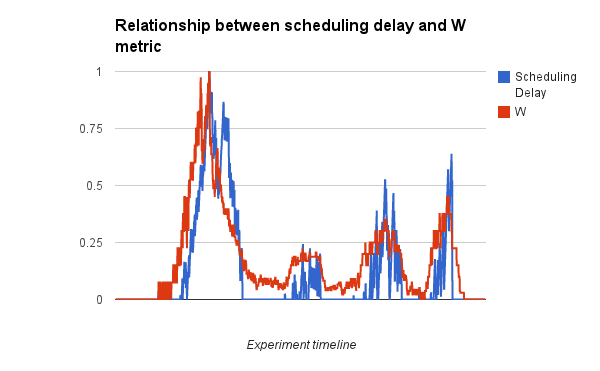
\includegraphics[width=\linewidth]{SchedulingDelay-W.png}
	\caption{The metric W correlates with scheduling delay}
	\label{fig:scheduling-W}
\end{figure}

\subsubsection*{Leasing and releasing policies}
To decide on scaling the system up or down, the state of the system is sampled in given intervals. The information gathered includes the amount of tasks in the queue, in each worker, the total number of cores available and the number of workers that have been requested but have not connected yet. With this information we construct a workload metric $W$, which, as seen in one of our experiments in \cref{fig:scheduling-W}, predicts the scheduling delay: $$W = tasks/cores$$ where $tasks$ is the set of all the tasks in the queue and the workers, and $cores$ are the total number of available cores in the workers. Generally, when $W > 1$, the system has been receiving jobs faster than it can process them, while $0 < W < 1$ means that the system has enough resources.

We use $W$ to decide on leasing or releasing more workers. Because one worker takes a significant amount of time to boot and $W$ can be expected to stay above $1$ while the resources are under way, we introduce the metric of \textit{promised workload} which also considers booting machines: 
$$PW = tasks/(cores + cores_{promised})$$
With this metric we avoid the situation that the system will repeat resource requests, because machines are not ready yet.

The last optimization we attempted was to lessen our system's responsiveness to request spikes. Since workers take a while to boot, it is possible that the spike is already served by the time the workers become available and thus the resources are not put to use. For that reason we reduce the responsiveness of the system using an exponential smoothing function
$$SPW_{i+1} = s*SPW_{i} + (1-s)*PW{i+1}$$ where $0 \leq s \leq 1$ is the smoothing factor. We've set $s=0.95$

We base our decisions for leasing and releasing machines on metric $SPW$. More specifically, we aim to keep it in $0.5 \leq SPW \leq 0.8$. When $SPW$ is below $0.5$ for a given amount of time, a machine is released. When $SPW$ is above $0.8$, a request for a $25$ increase is immediately performed. Note that our policy for scaling up is more aggressive than our policy for scaling down. There are two reasons for that decision. The first reason for that is that we choose to err on the side of having more resources than necessary. The second reason is that leasing resources is a slower operation. Once the workload is exceeds the system's capacity, jobs accumulate in the queue until more workers arrive. Even more resources will be needed to consume the queue and return the scheduling delays to acceptable levels. For that reason we also allow the system to issue multiple resource requests, even if the first batch of workers is still booting. The system will scale down again once the queue has been consumed.

\subsection{Additional System Features}
\label{subsec:additionalFeatures}
The additional feature covered in this prototype that was not required in the set of basic requirements is multi-tenancy. This term is defined as an IT sharing model of how physical and virtual resources are used by possibly concurrent tenants. In our application this means that multiple users can concurrently use the system, all connect to the head node, send in their workloads and all receive back their own result without seeing any results of other users.

In the research field of multi-tenancy, this brings up the philosophical question of fairness. Is it fair to discriminate between users that are very active and send in workloads more regularly than others or should a less active user have a higher priority? In this prototype we decided not to get into this discussion, just treating every user equal, using the policy of First-Come, First-Serve.

\section{Experiments}
\label{sec:experiments}
\textcolor{red}{1.5 pages}

\ldots

\subsection{Experimental setup}
\label{subsec:setup}
\textcolor{red}{Working environment (EC2), general workload and monitoring tools and other libraries}

Although the internal structures might differ, the general workings of all IaaS cloud services are mostly the same. Whether you choose for Amazon EC2, Microsoft Azure or another, the approach taken in the previous sections would be the same on architectural level. For this prototype we decided to use Amazon EC2, mainly because both authors already had good experience with it.

In order to lower the expenses on this project, we made use of the EC2 free tier machines. Each of our machines was an instance of a preconfigured Ubuntu t2.micro image. Computing resources for these virtual machines is done with a credit system that allows one to exceed its nominal performance, but suffer limits later on to make up for the burst. This was a significant problem for us, as the performance would plummet to less than 10\% of the burst. As an example, an image that is processed in 3 seconds in a burst, would take 40 to 60 seconds in  To make things even more complicated, the limits were applied per worker, which made worker performance very inconsistent. Our scheduling and scaling policies remained valid under the circumstances, but there is significant noise in our experiments nonetheless. We could not reduce the noise by averaging multiple experiments either, since the cause follows a strict pattern, starting with high performance and dropping shortly after. Another limitation to our experiments what that free-tier machines are limited to 20 at any given moment. This limited the scale of our experiments to use case that could be served by 20 machines with low performance.

In order to send tasks to the system for the purpose of experiments, we built a bot that sends tasks to the head node. With this we are able to send continuous streams of tasks (with user-defined intervals between requests) using a command line, as well as multi-tenant predefined experiments. 

We will present here two cases: in the first experiment, our system is surprised by a steady stream that exceeds its initial capacity. More specifically, the system starts with two workers available and the stream is one image every 2.5 seconds. With the processing times given earlier, we estimated that, with the worst performance by the workers, the system would need to scale 15 workers. In the second experiment, demand rises and falls over the course of a few minutes.

\subsection{Experimental results}
\label{subsec:results}
\textcolor{red}{Description of the experiments conducted to analyze each system feature, analyze them and describe the workload, present the operation of the system and analyze the results. See assignment}



\section{Discussion}
\label{sec:discussion}
\textcolor{red}{1 page - main findings, tradeoffs inherent in the design of cloud-computing-based applications.}

\section{Conclusion}
\label{sec:conclusion}
\textcolor{red}{\ldots}

%\bibliographystyle{abbrv}
%\bibliography{references}

\appendix
\section{Time sheet}
\label{app:time}
\textcolor{red}{table with time spend}
\end{document}